%% NOTES:

%REMOVE TOO HIGH LR! COLORS ARE REVERSE

%\begin{Imports and headers} 
%%%%%%%%%%%%%%%%%%%%%%%%%%%%%%%%%%%%%%%%%%%%%%%%%%%%%
\documentclass[a4paper]{article}  %Or use titlepage

%% Language and font encodings
\usepackage[english]{babel}
\usepackage[utf8x]{inputenc}
\usepackage[T1]{fontenc}
\usepackage{float} %makes you be able to use H option, places fig there and only there. VERY useful

%% Sets page size and margins
\usepackage[a4paper,top=3cm,bottom=2cm,left=3cm,right=3cm,marginparwidth=1.75cm]{geometry}

%% Useful packages
\usepackage{amsmath}
\usepackage{graphicx}
\usepackage[colorinlistoftodos]{todonotes}
\usepackage[colorlinks=true, allcolors=blue]{hyperref}

%% Header, foot and page number in bottom right corner
\usepackage{fancyhdr}
\usepackage{lipsum}

%% For long comments
\usepackage{comment} 

% Turn on the style
\pagestyle{fancy}
% Clear the header and footer
\fancyhead{}
\fancyfoot{}
% Set the right side of the footer to be the page number
\fancyfoot[R]{\thepage}
\fancyfoot[L]{\date{\today}}
\fancyhead[C]{DD2404 - Signal peptide prediction}

%\end{Imports and headers}

\begin{document}

%\begin{Title and abstract} 
%%%%%%%%%%%%%%%%%%%%%%%%%%%%%%%%%%%%%%%%%%%%%%%%%%%%
\title{\vspace{60mm} \bf 
Signal peptide prediction}  %Fix to center title vertically
\author{Timothy Bergström}
\maketitle
\thispagestyle{fancy}  %Page number for title (\maketitle clears foot and head, so it needs to be after it)
\newpage
\tableofcontents  %OBSOBS, you need to compile the document TWO TIMES for this to work. 
\newpage

\begin{abstract}
Detecting signal peptides (SPs) in proteins computationally is \dots
A neural network model was created and trained with X amount of data, which yielded a model with a classification accuracy of 92\% of the validation set.
The model was used to predict the total amount of SPs in the X and Y organism, which yielded Z and Q SPs respectively, showing that the model is \dots

%\lipsum[1]  % Fill with nonsense
\end{abstract}
%\end{Imports and headers} 

%\begin{Introduction} 
%%%%%%%%%%%%%%%%%%%%%%%%%%%%%%%%%%%%%%%%%%%%%%%%%%%%%

\section{Introduction}

Course bla. 

The goal is to create a classifier that can accurately classify proteins with \href{https://en.wikipedia.org/wiki/Signal_peptide}{signal peptides} (SPs) in an organisms \href{https://en.wikipedia.org/wiki/Proteome}{proteome}. 

SPs are short regions in peptides that are on average between 16 to 30 amino acids long, but can be as short as 8 and as long as 65 amino acids \cite{sp_length}. SPs function is to translocate proteins to different parts of the cell, such as insertion into membranes, moving proteins to organelles or to help the cell excrete the proteins \cite{sp_wiki}. 

\subsection{The structure of a signal peptide}

An SP is always located near the \href{https://en.wikipedia.org/wiki/N-terminus}{N-terminal} of a protein and have three regions; the n-region, the h-region and the c-region.

The n-region is the first region, which usually contains positively charged amino acids, making the region very polar and hydrophilic. Then comes the h-region, which contains mostly hydrophobic amino acids that forms an \href{https://en.wikipedia.org/wiki/Alpha_helix}{$\alpha$-helix} and lastly the c-region, which is usually a sequence of 3 to 8 non-charged polar amino acids. After the c-region, there is usually a cleavage site that have a tendency to be surrounded by small, uncharged amino acids.

When analyzing an organisms proteome, the SPs can give an indication where in the cell the proteins are translocated to which could be of an interest when researching an organism. Not all proteins contain SPs, which is why signal peptide prediction is useful for determining the layout of the cell and for annotating organisms proteomes. The problem with signal peptide prediction is that polar regions in trans-membrane proteins can mistakenly be predicted as the h-region of an SP, which makes predicting SPs in trans-membrane proteins difficult.

%\end{Introduction} 

%\begin{Methods and models}
%%%%%%%%%%%%%%%%%%%%%%%%%%%%%%%%%%%%%%%%%%%%%%%%%%%%%
\section{Methods and models}

\subsection{Design choices}
The neural network was written in python with Keras 2.0 and tensorflow 1.4 as the backend. The reason for using keras was that it can be used to quickly prototype and develop neural networks and with the tensorflow backend, a gpu can be used to run the calculations.

\subsection{Data sets}

A small sample of region-annotated proteins were provided by the course in \verb|fasta| format, containing mostly eukaryotic proteins. The samples also contained information if the proteins were transmembrane proteins or not. The data set contained both positive (contains a SP) and negative samples (does not contain a SP).
Some samples was extracted from NCBI ftp server, by extracting proteins annotated with signal peptide. Few positive samples and a large set of negative samples were obtained, mostly bacterial proteins.
Many of the positive samples were scraped from Signal Peptide database. A majority of the samples were bacterial proteins.
Most samples were extracted from Swissprot protein database. Mostly eukaryotic proteins, both negative and positive.

Proteomes from Homo sapiens, Mus musculus and Escherichia coli were obtained from Swissprot, a database of high-quality manually annotated proteins. 

\begin{table}[H]
\centering
\begin{tabular}{l | c | r} %If you add more columns, change here
Type & Positive & Negative \\\hline
TM & 10 & 30 \\
non-TM & 1 & 2 \\
Unknown & a & b
\end{tabular}
\caption{\label{tab:datatable}Data table.}
\end{table}

Typical signal peptide from dataset:
\begin{figure}[H]
\centering
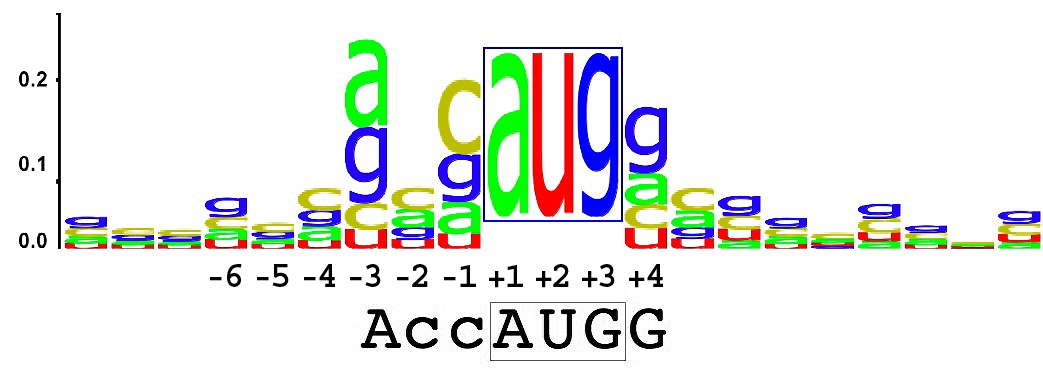
\includegraphics[width=0.7\textwidth]{pictures/seqlogo.png}
\caption{\label{fig:seqlogo}Extracted data from all positive samples}
\end{figure}

\subsection{Data preprocessing}

The protein sequences (samples) were contained in \verb|.fasta| files.
The first 30 amino acids from each sample were taken and sequences that were too short were padded with X.
First, the samples were cleared from all amino acids that were not one of the 20 standard amino acids. Unknown amino acids were labeled as X.
Each amino acids were then one-hot encoded (https://en.wikipedia.org/wiki/One-hot) and merged into one 2d array for each sample, creating a 3d array for all the samples.
Negative samples were labeled as 0 and positive samples were labeled as 1.
The data was lastly \href{https://en.wikipedia.org/wiki/Oversampling_and_undersampling_in_data_analysis}{undersampled}, making the ratio between negative and positive samples 50/50

\subsection{Neural Network structure}
The neural network was based on bidirectional \href{http://colah.github.io/posts/2015-08-Understanding-LSTMs/}{LSTMs}, due to LSTMs effectiveness with sequences and pattern recognition. \cite{rnn_effectiveness}. The bidirectionality of the network was added due to its success in other areas of machine learning with sequences and time-series predictions \cite{bidirectional_1} \cite{bidirectional_2}.

\begin{figure}[H]
\centering
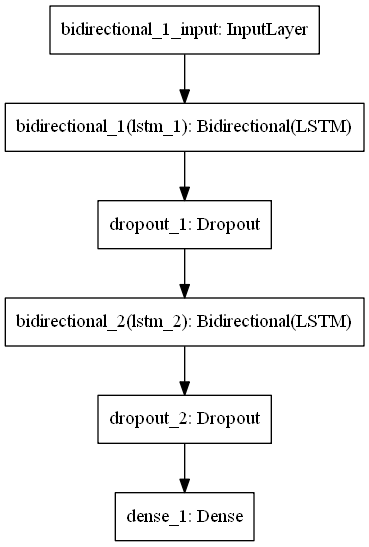
\includegraphics[width=0.7\textwidth]{pictures/model.png}
\caption{\label{fig:model_fig}Prediction model}
\end{figure}


\subsection{Related works}

There are multiple softwares and websites that predicts signal peptides, such as SignalP, SignalBlast and Predisi to name a few \cite{sp_predict1} \cite{sp_predict2} \cite{sp_predict3}. Neural Networks (NN) are the most used methods while some sites use Hidden Markov Models (HMM) instead. Similar methods are used to predict other biological problems, such as motifs and trans-membrane regions in proteins.

%\end{Methods and models}

%\begin{Evaluating model}
%%%%%%%%%%%%%%%%%%%%%%%%%%%%%%%%%%%%%%%%%%%%%%%%%%%%%
\section{Evaluating model}

\subsection{Model performance}
ROC-curve, CM-matrix for full data full data.

\subsection{Signal peptide detection in transmembrane proteins}
Evaluate transmembrane and non transmembrane acc/loss.
CM for TM and non-TM

\subsection{Signal peptide detection in proteomes}
Test two organisms, correct for CM

\subsection{Generative model}
A generative model was created that can create SPs. See in appendix \ref{GAN}.

%\end{Evaluating model}

%\begin{Conclusion}
%%%%%%%%%%%%%%%%%%%%%%%%%%%%%%%%%%%%%%%%%%%%%%%%%%%%%
\section{Conclusion}

Is it good enough? Can the model be improved? Can you use other methods (ex HMM, CNN, grouping etc...)

%\end{Conclusion}

%\begin{References}
%%%%%%%%%%%%%%%%%%%%%%%%%%%%%%%%%%%%%%%%%%%%%%%%%%%%%
\newpage
%% References
\bibliographystyle{alpha}
\begin{thebibliography}{9}

\bibitem{sp_length} Henrik Nielsen
\url{http://www.cbs.dtu.dk/services/SignalP-1.1/sp_lengths.html}

\bibitem{sp_wiki} Signal peptides wikipedia
\url{https://en.wikipedia.org/wiki/Signal_peptide}

\bibitem{rnn_effectiveness} ???
\url{http://karpathy.github.io/2015/05/21/rnn-effectiveness/}

\bibitem{bidirectional_1} ???
\url{https://web.stanford.edu/class/cs224n/reports/2760320.pdf}

\bibitem{bidirectional_2} ???
\url{http://www.cs.cmu.edu/afs/cs/user/zhouyu/www/ASRU.pdf}

\bibitem{sp_predict1} Henrik Nielsen,
 {\em Predicting Secretory Proteins with SignalP},
 In Kihara, D (ed): Protein Function Prediction (Methods in Molecular Biology vol. 1611),  pp. 59-73, Springer 2017, doi: 10.1007/978-1-4939-7015-5\_6, PMID: 28451972, 
\url{http://www.cbs.dtu.dk/services/SignalP/}  %CHAR _ makes Latex crash, use \_

\bibitem{sp_predict2} Karl Frank; Manfred J. Sippl,
{\em High Performance Signal Peptide Prediction Based on Sequence Alignment Techniques},
Bioinformatics, 24, pp. 2172-2176 (2008), \url{http://sigpep.services.came.sbg.ac.at/signalblast.html}

\bibitem{sp_predict3}  Karsten Hiller,
{\em PrediSi}, Institute for Microbiology Technical University of Braunschweig, 
\url{http://www.predisi.de/}

\end{thebibliography}

%\end{References}

%\begin{Appendix}
%%%%%%%%%%%%%%%%%%%%%%%%%%%%%%%%%%%%%%%%%%%%%%%%%%%%%
\newpage

\section{Appendix}

\subsection{Training the model}
Train time, gpu used, specs, time to train etc...
Gpu is needed to improve training speed. Add epoch time for gpu and cpu

Everything that the person reading don't want to know


\subsection{Model details}

??

\subsection{Pitfalls when training a model}
Concept of under and overfitting and how to prevent it. Example pictures of bad models.

Overfitting \dots

other stuff too

more stuff

\begin{figure}[H] %Rank in order
\center
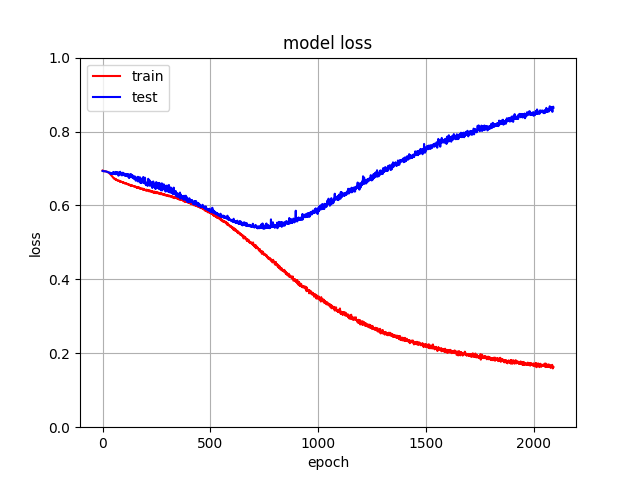
\includegraphics[width=0.7\textwidth]{pictures/overfit.png}
\caption{\label{fig:overfit}Overfitted}
\end{figure}

Too high learning rate \dots

other stuff too

more stuff

\begin{figure}[H]
\center
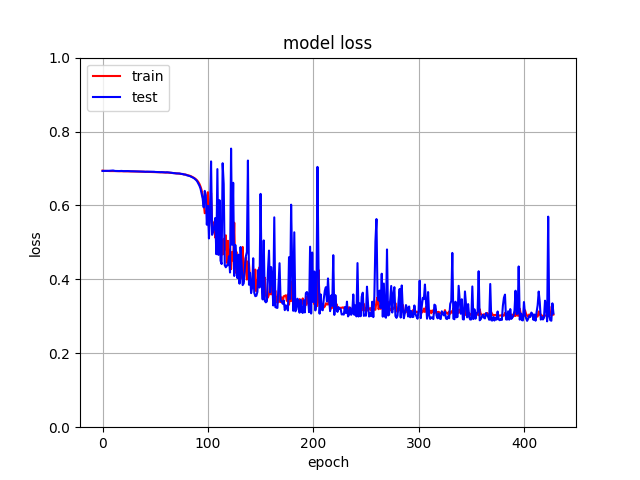
\includegraphics[width=0.7\textwidth]{pictures/high_lr.png}
\caption{\label{fig:high_lr}Too high learning rate}
\end{figure}


\subsection{Additional features}

Loading the data can be used in many ways. One way is to augment the data by dividing each sequence into many chunks, taking the chunk closest to the N-terminal as positive and the rest as negative.

Due to the large amount of data obtained, data augmentation were not used.

Advantages with data augmentation: 
Each positive sample would yield multiple negative samples, so smaller data sets can be used for training.
Using positive samples and the negative samples from different organisms could make the model overfit to a particular amino acid bias. Using other regions of the positive samples would preserve the amino acid bias, making the data more consistent.
Some trans-membrane regions of the proteins might be very similar to signal peptide regions, which would force the model to improve the prediction of trans-membrane proteins. 

Disadvantages with data augmentation:
The first amino acid in the N-terminal has an extremely high bias towards some amino acids, mainly Methionine, see Figure~\ref{fig:seqlogo}. The model would then have a high affinity for the first amino acids, creating a poor model that would only detect if the sequence is located in the N-terminal or not. The first amino acids of each sequence were removed, so the this would not be a problem.
The N-terminal of peptides both with and without SPs might have a similar structure compared to other regions of protein, which would make the model as stated above, only be able to distinguish if the region is at the N-terminal or not. To prevent this problem, both negative samples from the N-region and other regions of the proteins could be used.


\subsection{Generative Model} \label{GAN}


%\end{Appendix}

\end{document}


%\begin{DUMP}

\begin{comment}

\LaTeX{} is great at great tool. Let $X_1, X_2, \ldots, X_n$ be a sequence of independent and identically distributed random variables with $\text{E}[X_i] = \mu$ and $\text{Var}[X_i] = \sigma^2 < \infty$, and let
\[S_n = \frac{X_1 + X_2 + \cdots + X_n}{n} = \frac{1}{n}\sum_{i}^{n} X_i\]
 $n$ approaches infinity, the random variables $\sqrt{n}(S_n - \mu)$ converge in distribution to a normal $\mathcal{N}(0, \sigma^2)$.

List of things \dots
\begin{enumerate}
\item Problems,
\item Structure data
\end{enumerate}
\dots More things \dots
\begin{itemize}
\item Things to add,
\item Testing
\end{itemize}

\end{comment}

%\end{DUMP}
